
\chapter{Prestatie verwachtingen}
\label{Prestatie_verwachtingen}
\textit{In dit hoofdstuk worden de prestaties verwachtingen toegelicht aan de hand van de in \cref{cha:opdrachtanalyse} opgestelde prestatie criteria (\cref{se:PC}) en functionele eisen (\cref{se:PVE}). In \cref{se:presentatie_ontwerp} wordt het ontwikkelde concept gepresenteerd, hier wordt een korte omschrijving van het ontwerp gegeven samen met een afbeelding. In \cref{se:prestatie_en_eigenschappen} worden de verwachte prestaties verteld met eventuele berekeningen om dezen te ondersteunen, ook worden hier de specifieke eigenschappen van het ontwerp toegelicht. In \cref{se:veiligheidsanalyse_prestatieverwachting} wordt een veiligheid-overzicht van het ontwerp gepresenteerd.}

\section{Presentatie van het ontwerp}
\label{se:presentatie_ontwerp}

De Driepoter is een ontwerp dat in staat is om over obstakels heen te stappen door middel van zijn inklapbare poten. Zoals te zien is in \cref{fig:De_driepoter_Prestatie_analyse} is de Driepoter in staat om de schaarliften die hij aan de onderkant van het chassis heeft in te klappen en uit te klappen. De Driepoter kan het pakket ontvangen door middel van een rol-baar plateau, dit zorgt ervoor dat de Drieklapper een verstelbaar zwaarte punt heeft wat handig is voor het nemen van een talud. Eenmaal wanneer de Driepoter een bocht moet maken kan hij zien voorste wielen draaien en net als een auto een bocht maken.\\

\vspace{\baselineskip}
\begin{figure}[H]
    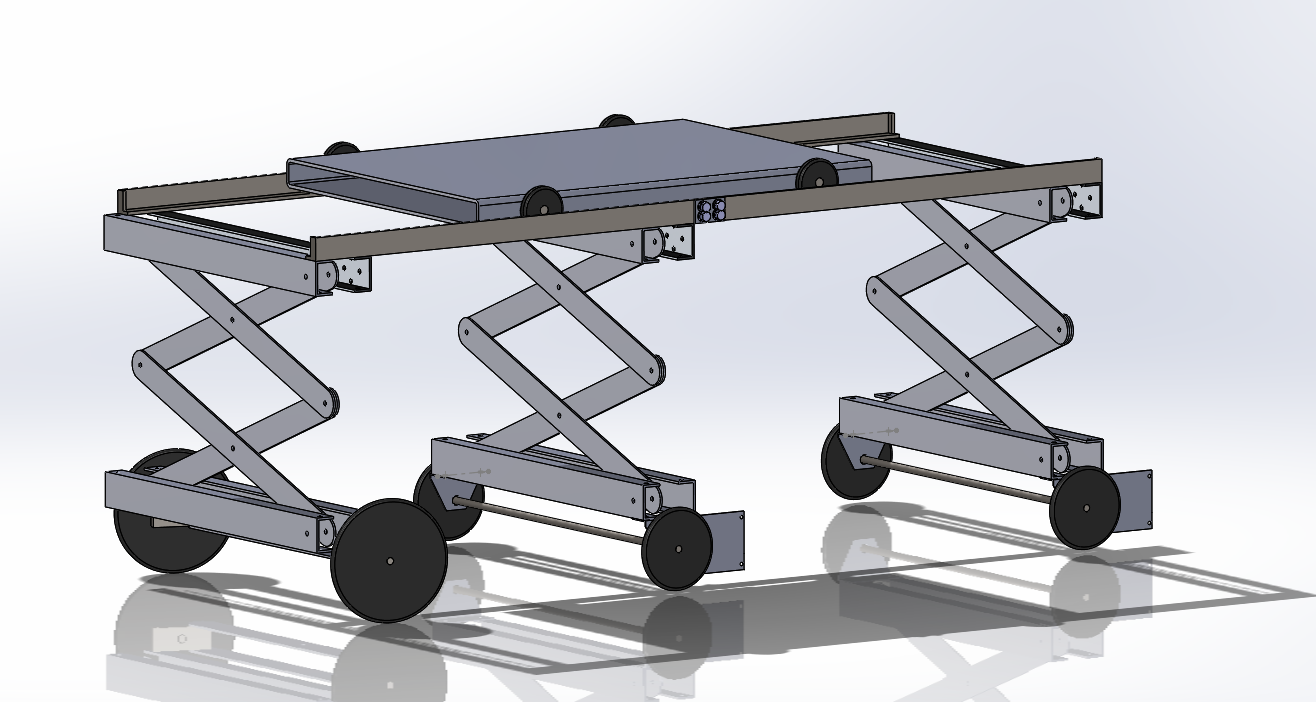
\includegraphics[width = 120mm]{04_gekozenconcept/eindconcept.png}
    \caption{de Driepoter}
    \label{fig:De_driepoter_Prestatie_analyse}
\end{figure}


\section{Verwachte eigenschappen en prestaties}
\label{se:prestatie_en_eigenschappen}
Hier worden de prestaties en de eigenschappen van de Driepoter besproken en onderbouwt door middel van berekeningen en bronnen. De mogelijke prestaties zijn aan de hand van de prestatie criteria en het programma van eisen in \cref{cha:opdrachtanalyse} opgesteld. De gekozen prestaties en eigenschappen die moet worden bepaald zijn: De dynamische en statische stabiliteit, het balans van het pakketje, de benodigde hoeveelheid energie voor het nemen van de hindernis baan en de tijd die het pakket hondje kost voor het nemen van de hindernisbaan. 

\subsection{De stabiliteit}
Erg belangrijk is het voor het pakkethondje dat hij niet omvalt tijdens het versnellen, afremmen of het nemen van een talud. De stabiliteit is in twee delen verdeeld: de dynamische stabiliteit en de statische stabiliteit. Onder de dynamische stabiliteit valt het versnellen en remmen van het pakkethondje en onder de statische stabiliteit valt het nemen van een talud en het rijden van het pakkethondje.\\
Voordat er berekeningen worden gedaan moeten een aantal parameters worden bepaalt:

\begin{itemize}
    \item \textbf{De hoogte van het massamiddelpunt bij verschillende tijdstippen in het nemen van de hindernisbaan}. De hoogte van het massa middelpunt als de schaarliften volledig zijn ingeklapt is 
    \item \textbf{Het steunvlak}. Deze wordt bepaald door de 3 paar wielen aan de onderkant van de schaarlift. De wielen staan 530 mm en 350mm van elkaar af. 
    \item Eventuele externe krachten of veranderingen in deze krachten
    \item Maximale hoek van talud 1
    \item De maximale versnelling
\end{itemize}
\vspace{\baselineskip}

\subsection{Balans van het pakketje}

\subsection{Benodigde hoeveelheid energie}

\subsection{Snelheid van het nemen van de hindernisbaan}


\section{veiligheidsanalyse}
\label{se:veiligheidsanalyse_prestatieverwachting}

